\newcommand{\beginsupplement}{%
%	\setcounter{table}{0}
%	\renewcommand{\thetable}{S\arabic{table}}%
	\setcounter{figure}{0}
	\renewcommand{\thefigure}{S\arabic{figure}}%
}

\beginsupplement
\section{Supplemental}

\begin{figure*}[ht]
	\centering
	%	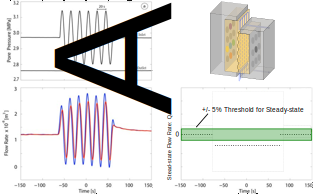
\includegraphics[width=1.0\columnwidth]{PpFlow_fig_v1}
	%	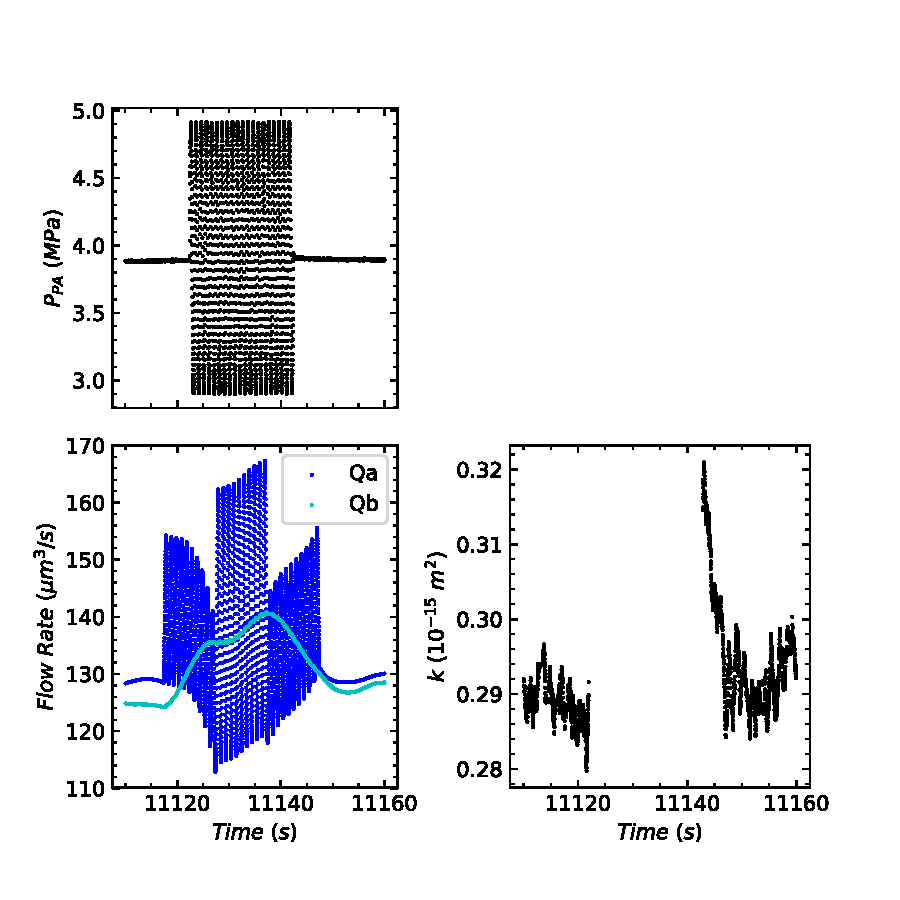
\includegraphics[width=0.8\columnwidth]{permCalcPlots_p4975_run3b_1Hz}
	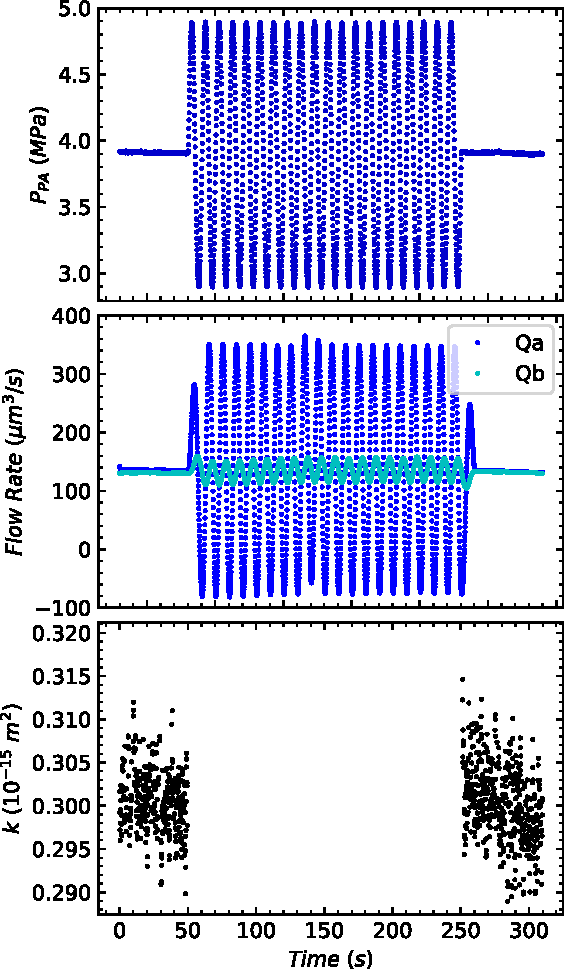
\includegraphics[width=0.4\columnwidth]{permCalcPlots_tall_p4975_run3b_1Hz}
	\caption[]{Example of dynamic stressing and the corresponding flow rate measurements for a set of pore pressure oscillations in experiment p4975. Note that the plots (a) and (b) are decimated for clarity. (a) Imposed pore pressure oscillation at inlet and fixed pore pressure at the outlet. Pressure conditions before and after the oscillations are identical. (b) Measured flow rates at the fracture inlet (blue line) and outlet (red dashed line). Notice the small time lag ($\leq$ 2 s) between the maxima of the inlet and outlet flow rates. (c) Permeability at steady-state and during the pore pressure oscillation. In the calculation of permeability we impose a threshold between the flow rates to ensure steady-state flow ($Q_{A} - Q_{B}  \leq 5 \% $). It is reasonable to assume that even at relatively low frequency oscillations, there is effectively no steady-state flow during the imposed oscillations.}
	\label{fig:perm_calc}
\end{figure*}

\textcolor{red}{We measure the effective permeability, ka, by calculating the flow rate over a 2 s window. For pore pressure oscillations, we start 10 s after the oscillation to ensure that permeability measurement is not affected by the Pp oscillation and/or by storage effects. Need to annotate Flow Rate with lines indicating the +- 5\%}

\newpage


%\begin{figure}[ht]
%	\centering
%	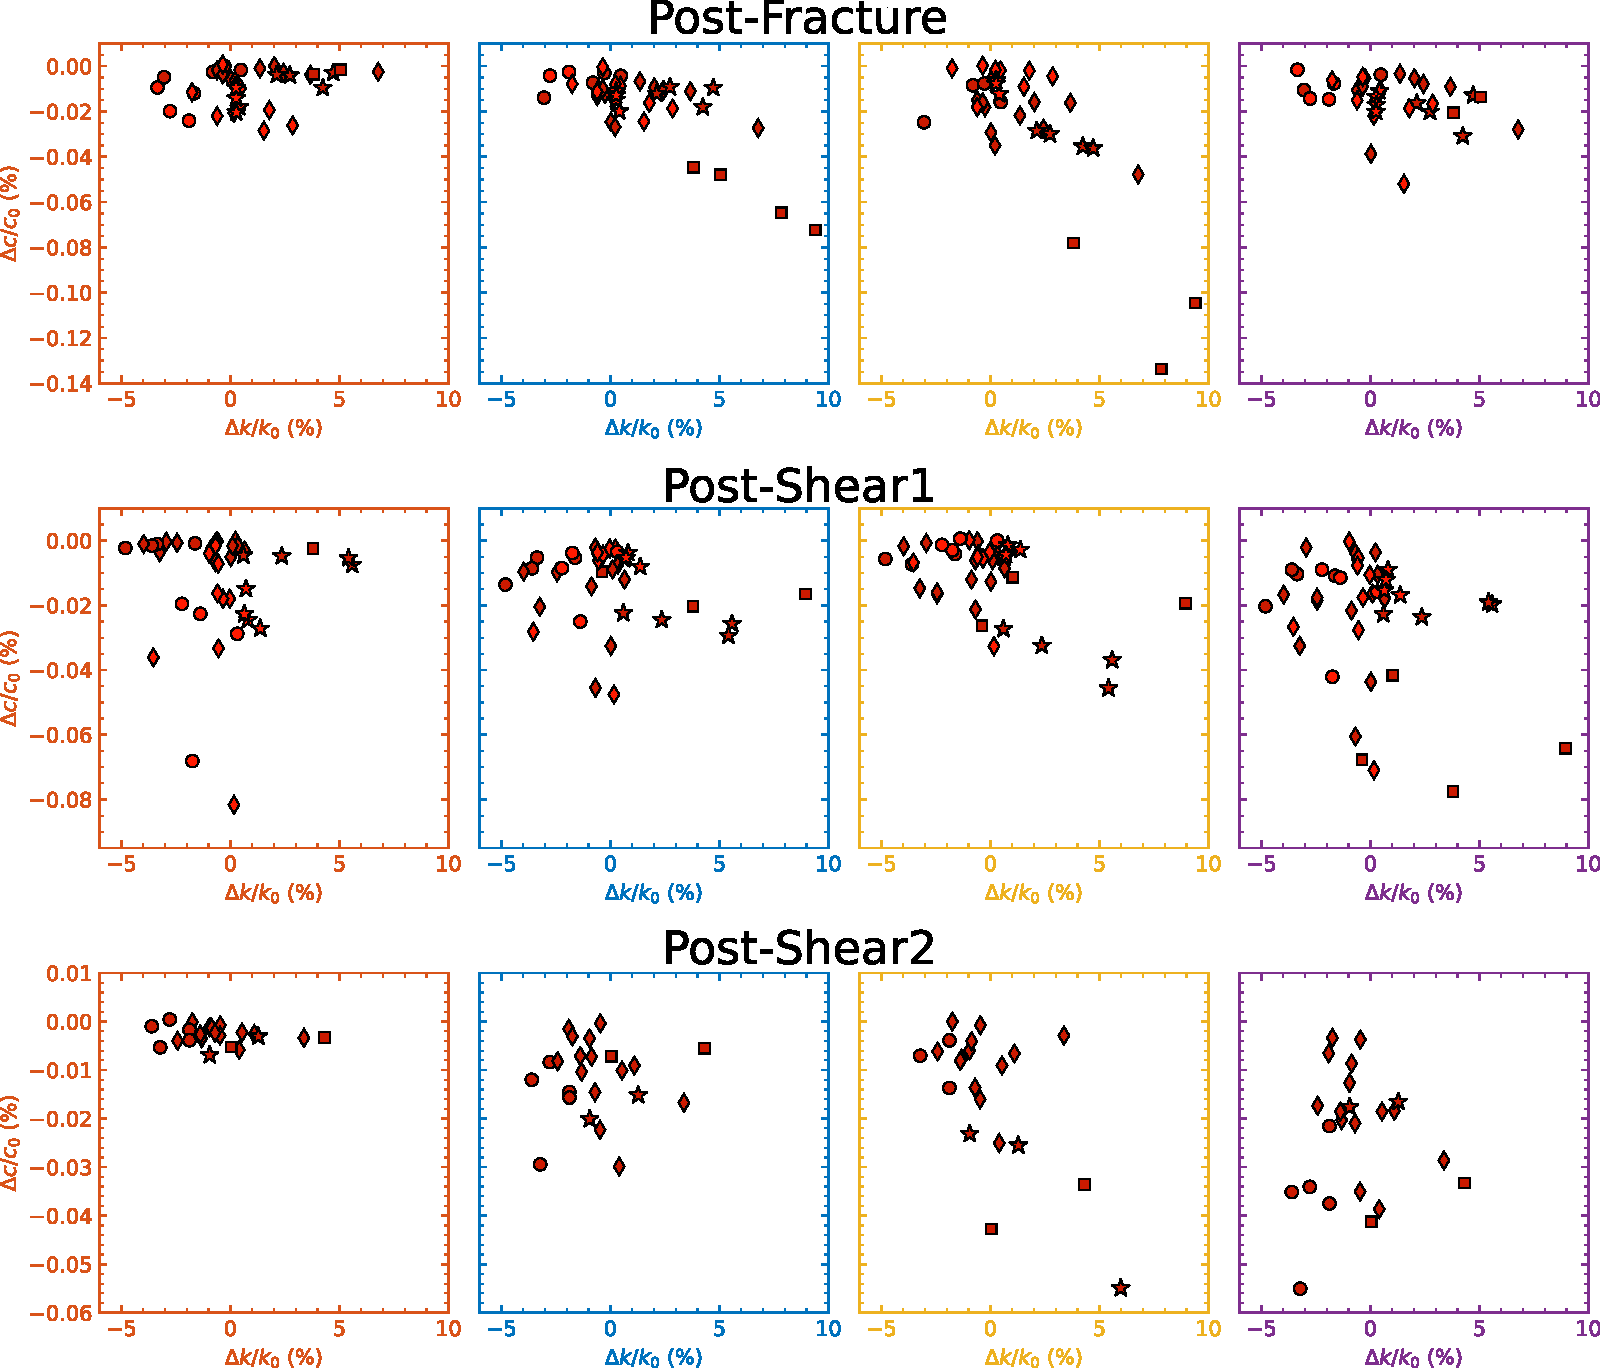
\includegraphics[width=1\columnwidth]{Delc_all_NS_all}
%	%\enspace
%	%\includegraphics[width=6cm]{post-frac_amp_array}
%	\caption{Nonlinearity as a function of permeability change for $ \sigma_{NS} $ oscillations for each receiver. Transitioning from post-fracture results to post-shear results, we observe decreased nonlinearity and permeability enhancement. This is probably related to clogging mechanisms.}%
%	\label{fig:delc_plots_ns}
%\end{figure}
%
%\newpage
%
%\begin{figure}[ht]
%	\centering
%	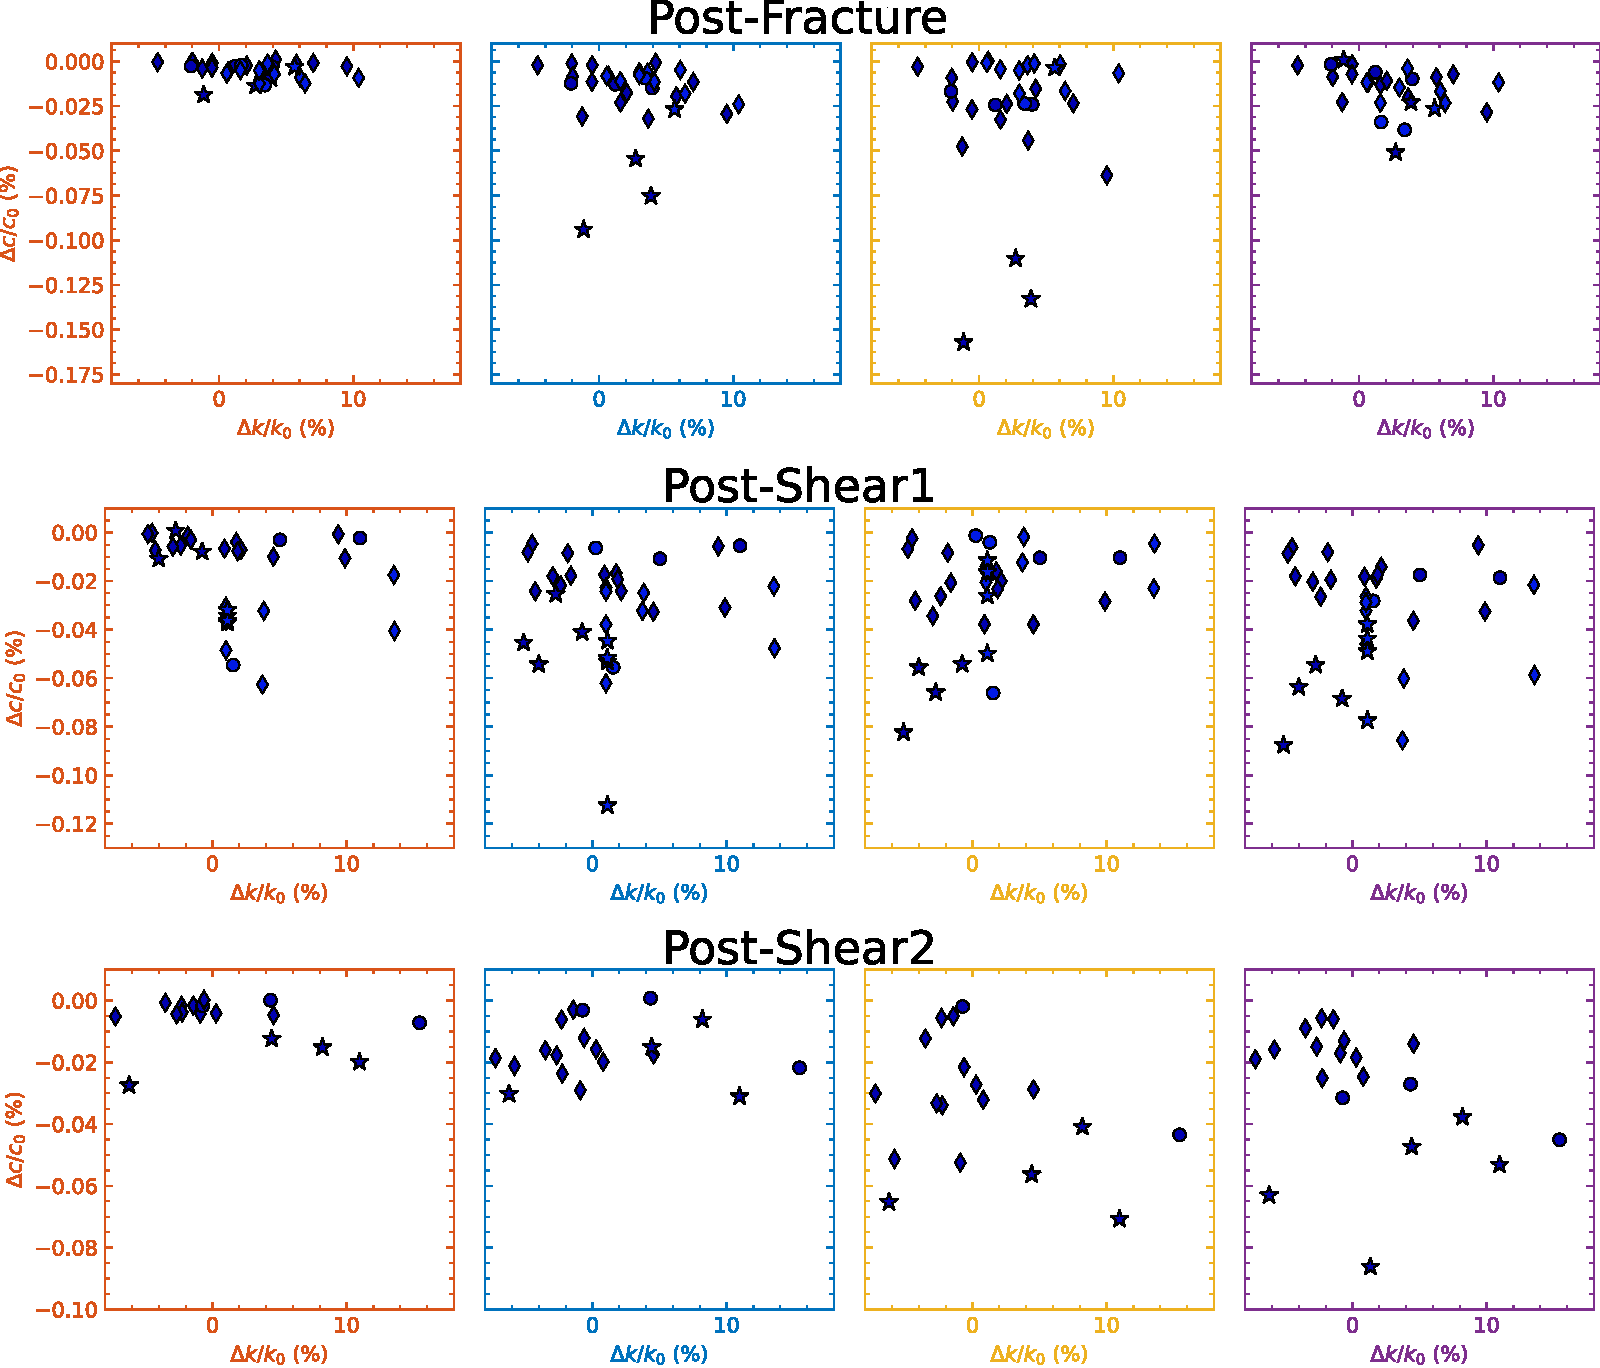
\includegraphics[width=1\columnwidth]{Delc_all_PP_all}
%	%\enspace
%	%\includegraphics[width=6cm]{post-frac_amp_array}
%	\caption{Nonlinearity as a function of permeability change for $ P_P $ oscillations for each receiver.}
%	\label{fig:delc_plots_pp}
%\end{figure}

\newpage

\begin{figure}[ht]
	\centering
	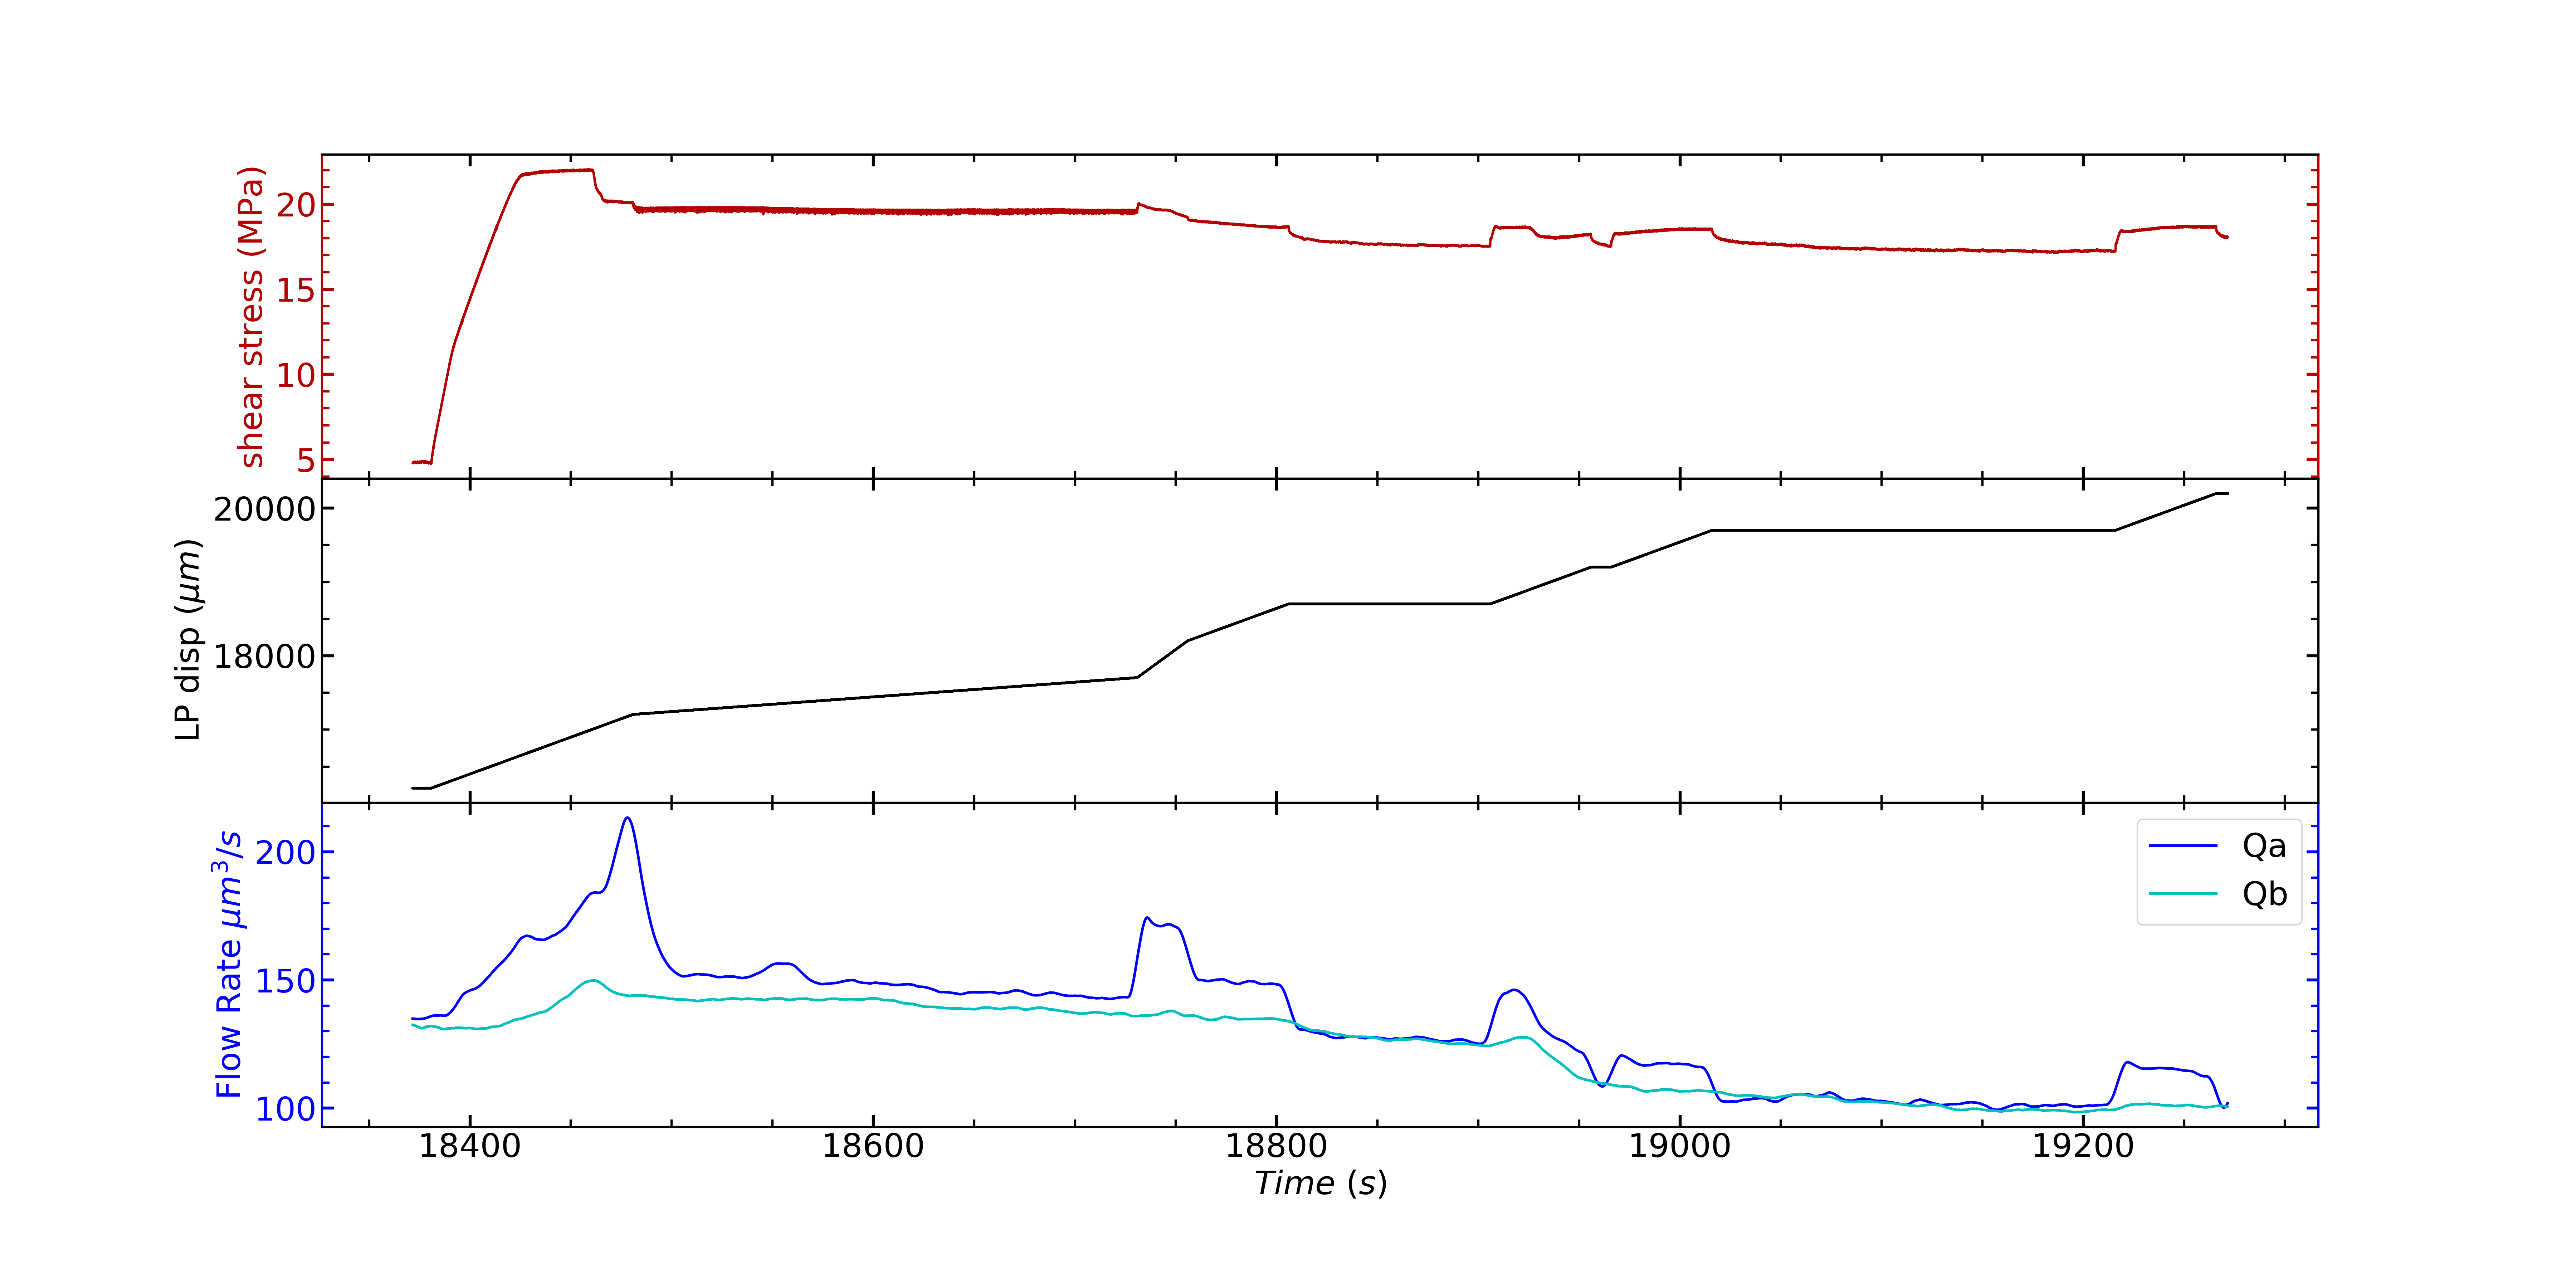
\includegraphics[width=1\columnwidth]{Shearing_p4975_shr1}
	\caption{First shearing for p4975.}
	\label{fig:shr1_p4975}
\end{figure}

\newpage

\begin{figure}[ht]
	\centering
	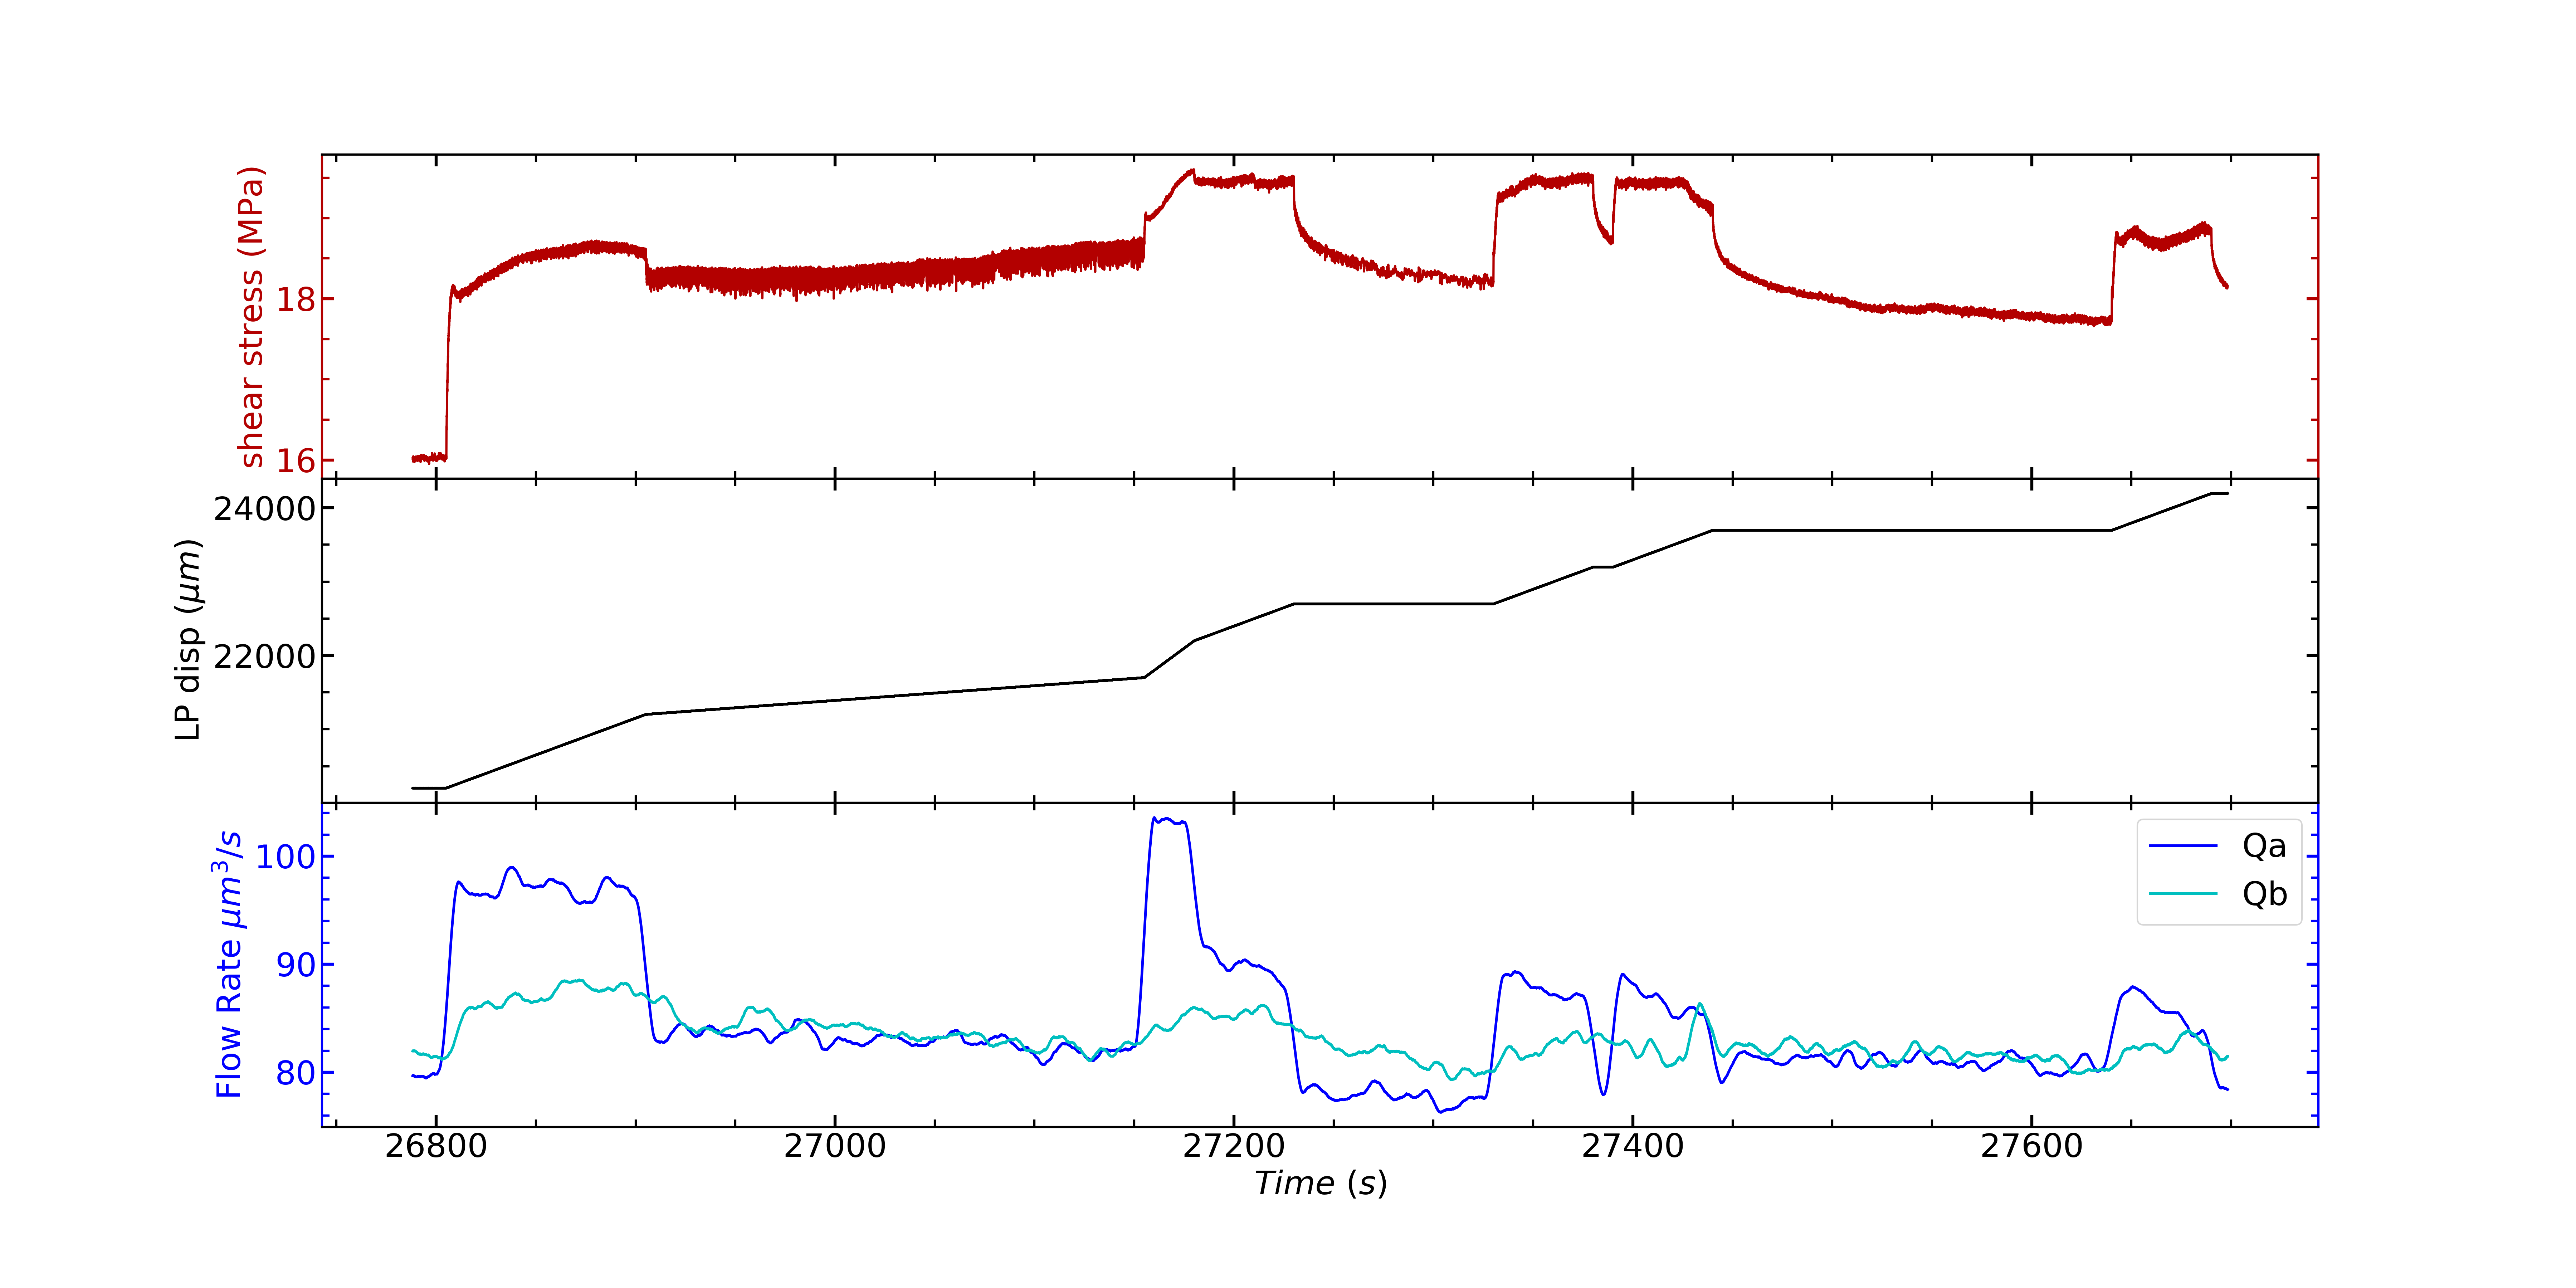
\includegraphics[width=1\columnwidth]{Shearing_p4975_shr2}
	\caption{Second shearing for p4975.}
	\label{fig:shr2_p4975}
\end{figure}

%++++++++++++++++++++++++++++++++++++++++
% References section will be created automatically 
% with inclusion of "thebibliography" environment
% as it shown below. See text starting with line
% \begin{thebibliography}{99}
% Note: with this approach it is YOUR responsibility to put them in order
% of appearance.